\section{Gateway}
In this section, we describe a SCION gateway, which bridges between a SCION network and an IP network. SCION gateways enable (1) connecting two physically separate SCION networks via IP networks, and (2) IP clients to communicate with/through a SCION network without modifying their protocol stack (i.e., transparently). In essence, SCION gateways integrate SCION networks with IP networks in a seamless manner, thereby enabling incremental and independent adoption of SCION architecture. 

\begin{figure*}[ht]
\centering
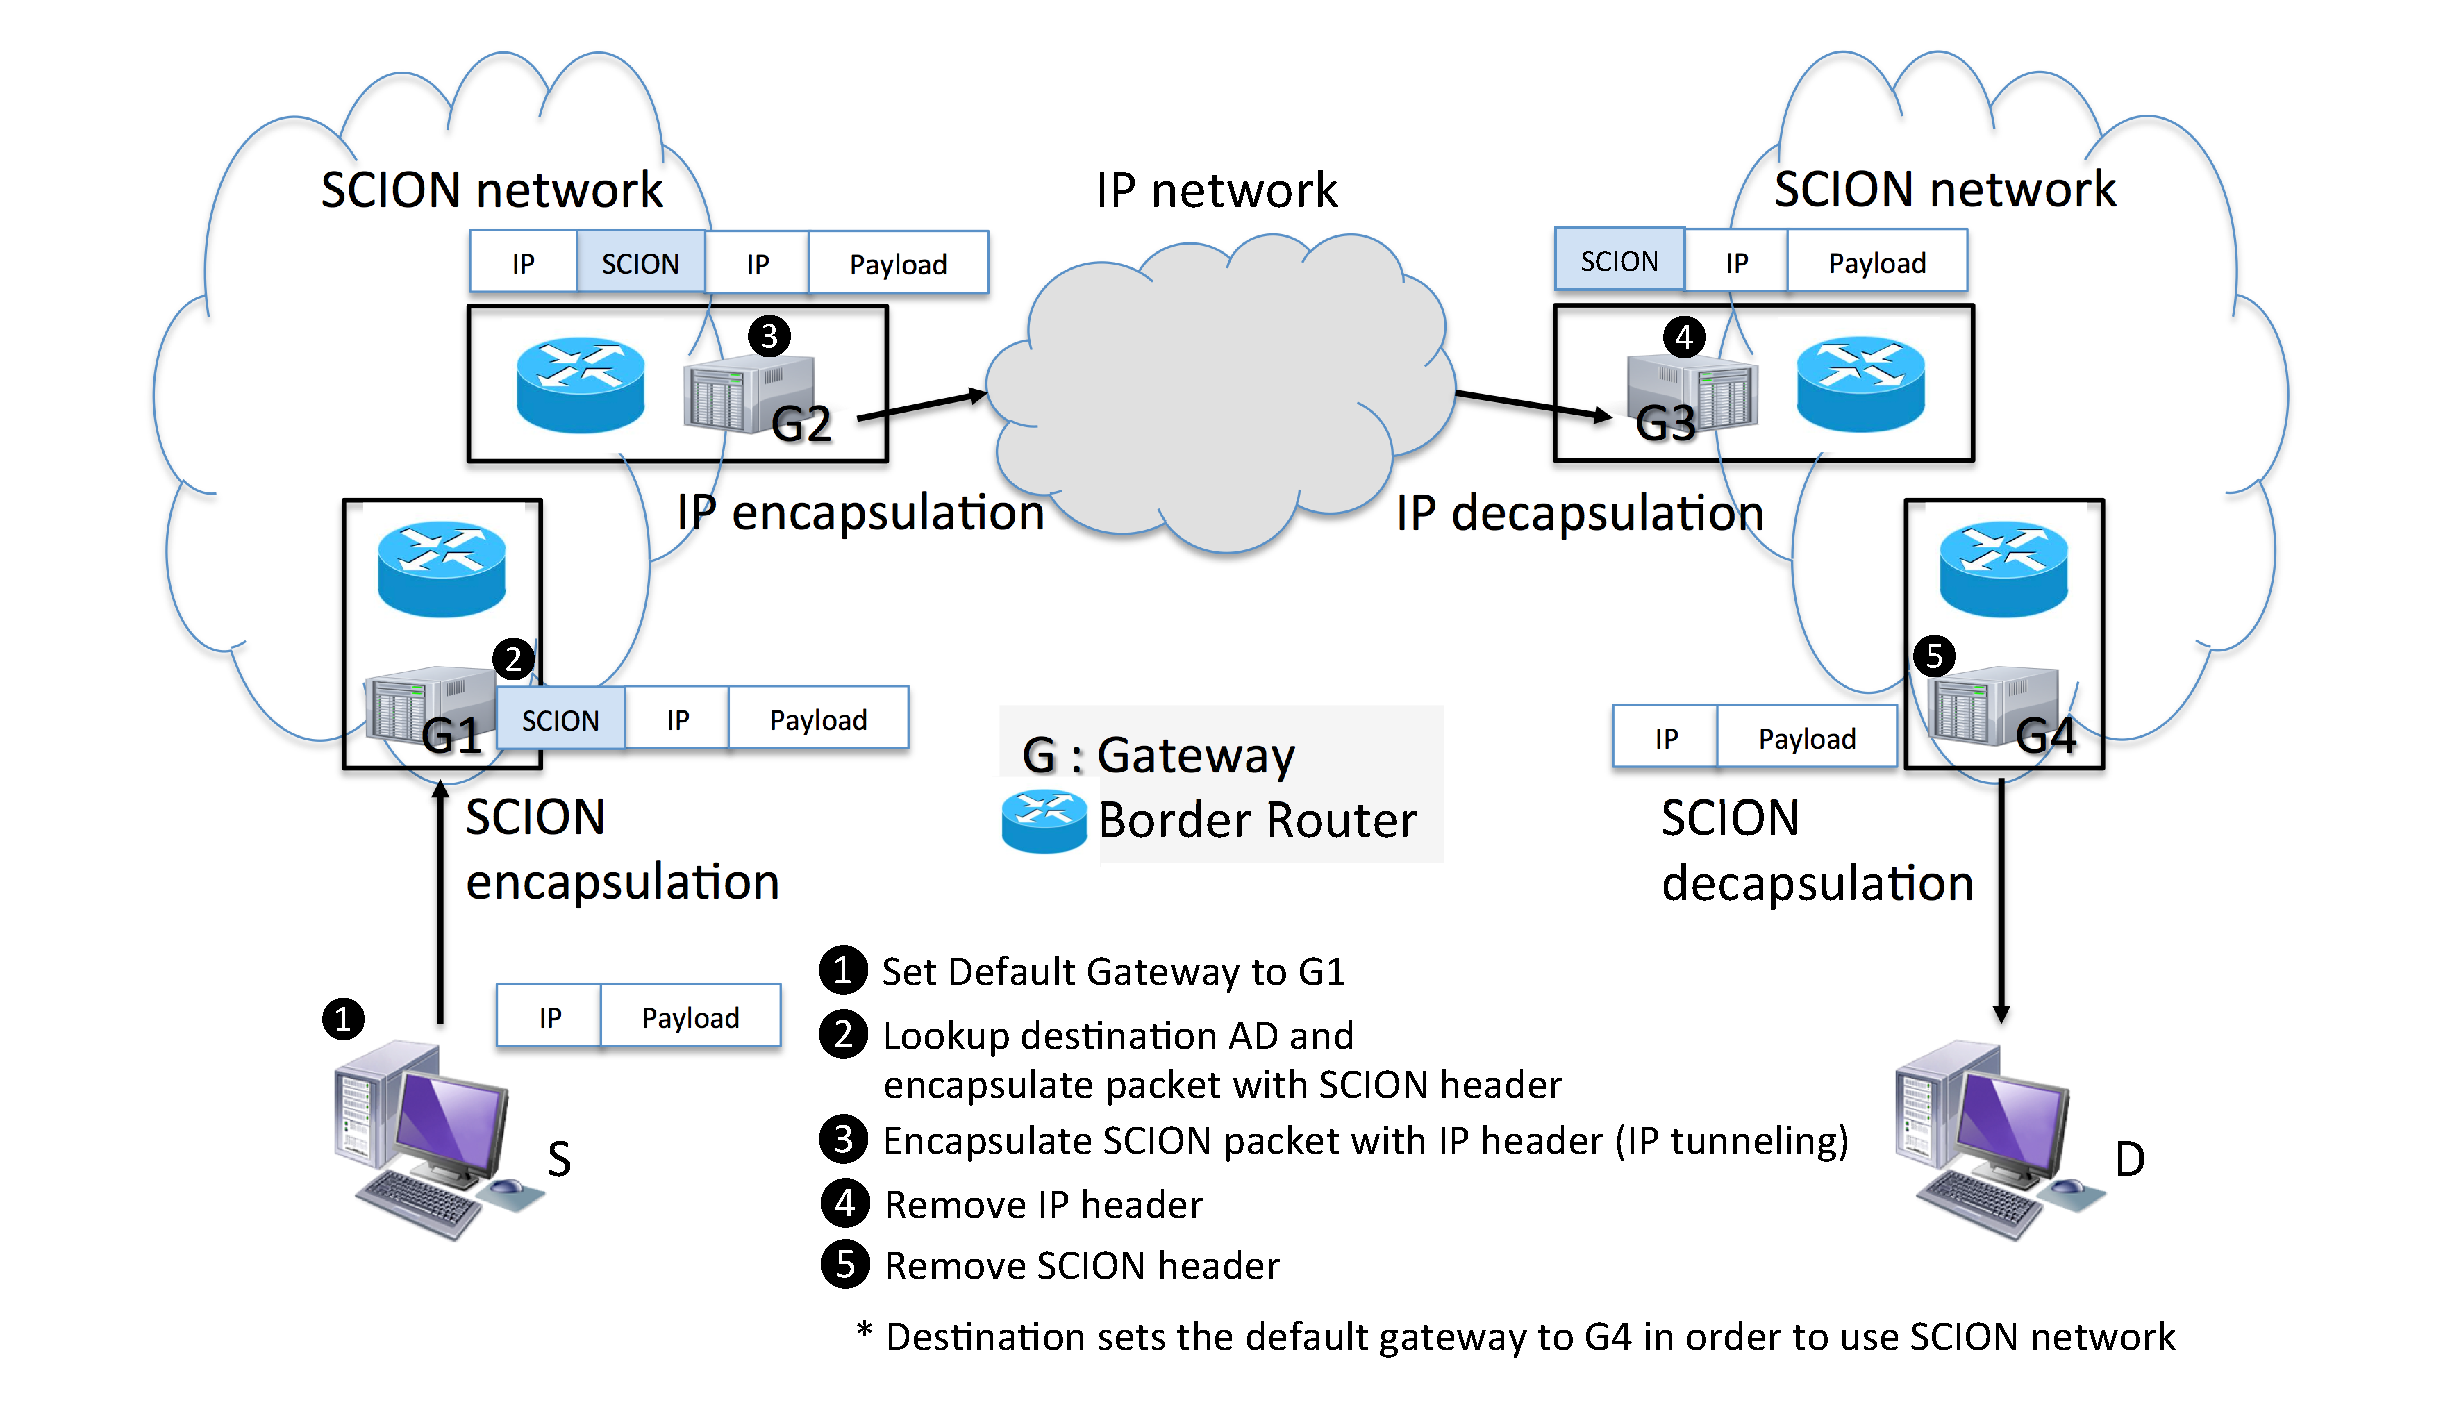
\includegraphics[width=\columnwidth]{./fig/gateway.eps}
\caption{SCION Gateway.}\label{fig:gateway}
\end{figure*}

\subsection{Gateway for IP tunneling}
Two SCION networks can be connected via IP network using SCION gateways. For this purpose, SCION gateways encapsulate a SCION packet with IP header, where the sending gateway sets the source IP address to its own address and the destination IP address to that of receiving gateway. Once a SCION gateway receives a packet from another SCION gateway~\footnote{Each gateway has the list of SCION gateways in its configuration file}, it removes IP headers and forward packet to the SCION network to which it is connected. That is, SCION gateways have at least two interfaces that are connected to two different networks (i.e., SCION and IP networks) and forward SCION packets through {\em IP tunnels}. Tunneling is simply configured as: the sending gateway has the map between an outgoing SCION interface (to itself) and the IP address of the corresponding destination gateway to which the incoming SCION interface is connected; the receiving gateway has the list of the IP addresses of sending gateways.The receiving gateway, once it removes a packet's IP header, is able to determine the SCION interface to which the packet should be place. We name this type of gateway as {\em IP tunneling} SCION gateway. The steps 3 and 4 in figure~\ref{fig:gateway} illustrate this IP tunneling. 

\subsection{Gateway for IP clients}
All IP-based applications can communicate via SCION network by setting their default gateway to the IP address of SCION gateway. For this purpose, SCION gateways, on receiving a packet from the IP interface, look at the destination address of the packet, resolve the address to the destination AD, and encapsulate the IP packet with the SCION header. As a result, this gateway, named {\em last-mile gateway}, enables IP clients to use SCION networks without changing its protocol stack. The destination gateway simply removes the SCION header and forward the packet to the destination address in the IP header. In this case, the whole IP packet is treated as a payload by SCION routers and only is interpreted by {\em last-mile} SCION gateways. Steps 2 and 5 in Figure~\ref{fig:gateway} illustrate packet processing by the last-mile SCION gateways.

